\newpage
\section{Auswertung}
\label{sec:evaluation}
\subsection{Mikrostruktur}
Die Originaldaten der Messung der Kreisstruktur sind in Abbildung \ref{fig:KREIS1} dargestellt. 
Im Vergleich sind die Messungen mit und ohne Strain-Gauge-Nachregelung zu sehen.

\begin{figure}[H]
    \centering
    \begin{subfigure}{0.49\textwidth}
        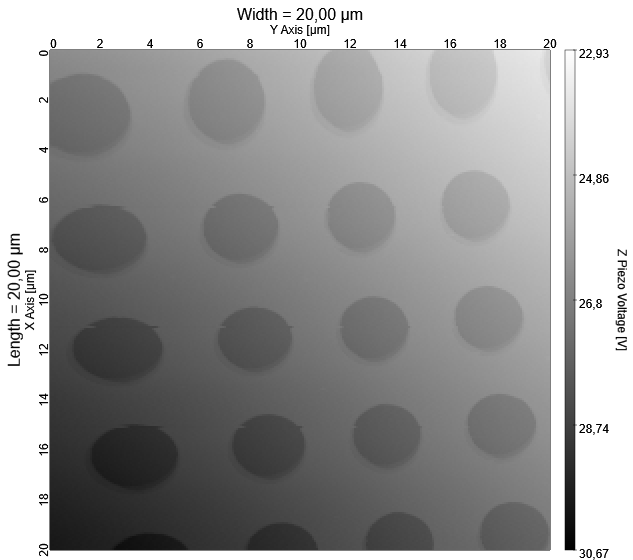
\includegraphics[width=\textwidth]{bilder/Mikrostruktur/Kreis2_Res250px_Speed100pps_ohne_Nachregelung_withscale.png}
        \caption{}
        \label{fig:A1}
    \end{subfigure}
    \begin{subfigure}{0.49\textwidth}
        
\includegraphics[width=\textwidth]{bilder/Mikrostruktur/Kreis2_Res250px_Speed100pps_withscale.png}
        \caption{}
        \label{fig:A2}
    \end{subfigure}
    \caption{Originaldaten des Vorwärtsscans der Mikrostruktur im Bereich der Kreisstruktur. \textbf{(a)} Ohne Strain-Gauge-Nachregelung, \textbf{(b)} mit Strain-Gauge-Nachregelung.}
    \label{fig:KREIS1}
\end{figure}


Für eine verbesserte Darstellung wurden die Daten mit Gwyddion \cite{Gwyddion} bearbeitet. In Abbildung \ref{fig:KREIS2} sind 
die bearbeiteten Datensätze jeweils für den Vorwärts- und Rückwärtsscan dargestellt. Dabei wurden die Werte invertiert, eine Ebenensubtraktion und 
Zeilenkorrektur vorgenommen. Außerdem wurde zur Präsentation ein farbiger Gradient verwendet, mit einer Darstellung in 2 und 3 Dimensionen.

\begin{figure}[H]
    \centering
    \begin{subfigure}{0.49\textwidth}
        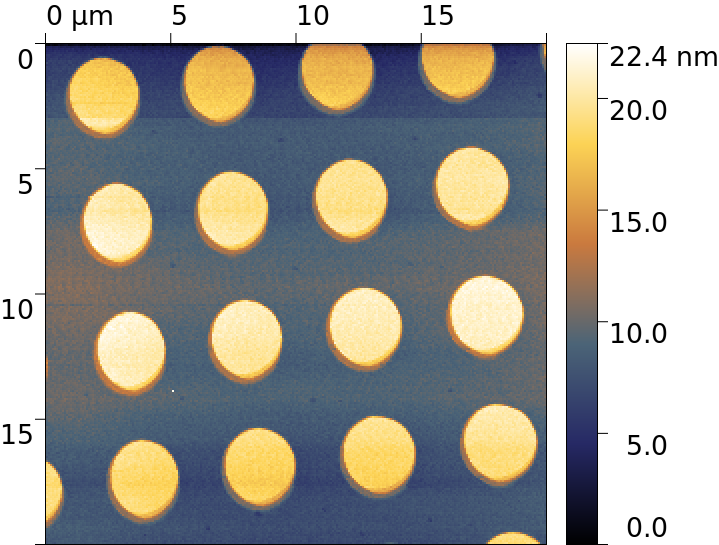
\includegraphics[width=\textwidth]{bilder/Mikrostruktur/Kreis_Vor_2D.png}
        \caption{}
    \end{subfigure}
    \begin{subfigure}{0.49\textwidth}
        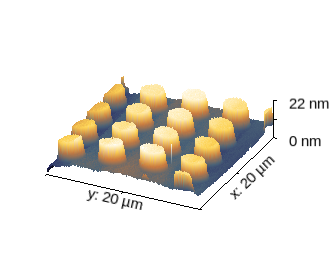
\includegraphics[width=\textwidth]{bilder/Mikrostruktur/Kreis_Vor_3D.png}
        \caption{}
    \end{subfigure}
    \begin{subfigure}{0.49\textwidth}
        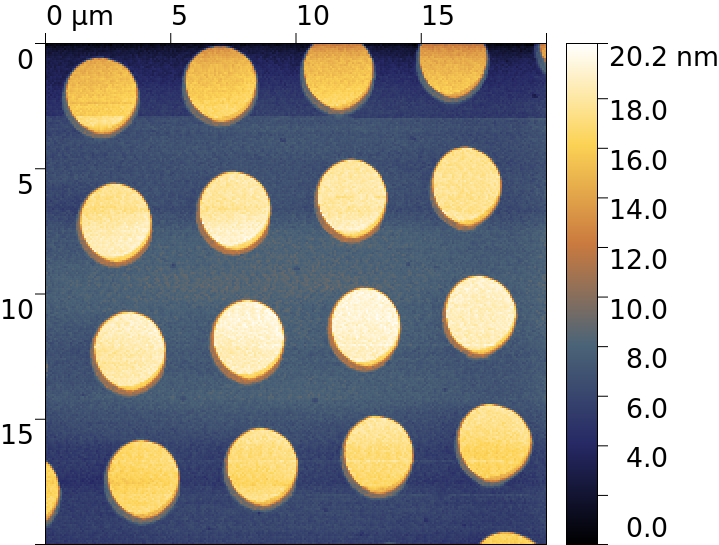
\includegraphics[width=\textwidth]{bilder/Mikrostruktur/Kreis_Bac_2D.png}
        \caption{}
    \end{subfigure}
    \begin{subfigure}{0.49\textwidth}
        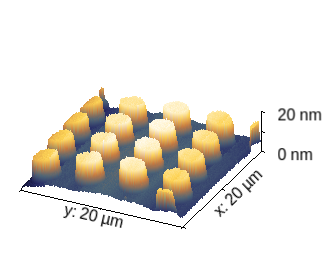
\includegraphics[width=\textwidth]{bilder/Mikrostruktur/Kreis_Bac_3D.png}
        \caption{}
    \end{subfigure}
    \caption{Mit Gwyddion aufbereitete Daten der Kreisstruktur. \textbf{(a)} Vorwärtsscan in 2D Darstellung, \textbf{(b)} Vorwärtsscan in 3D Darstellung, \textbf{(c)} Rückwärtsscan in 2D Darstellung, \textbf{(d)} Rückwärtsscan in 3D Darstellung.}
    \label{fig:KREIS2}
\end{figure}
Um die Strukturabstände zu bestimmen, wurden Linienprofile entlang der Kreise genommen, 
jeweils in x- und y-Richtung für alle vollständig sichtbaren Strukturen. Ein Beispiel für ein solches Linienprofil ist in Abbildung \ref{fig:KREISE3}
zu sehen. Mittels der 'Measure Distances'-Funktion von Gwyddion konnten so die Distanzen zwischen einzelnen Punkten ermittelt werden.
\begin{figure}[H]
    \centering
    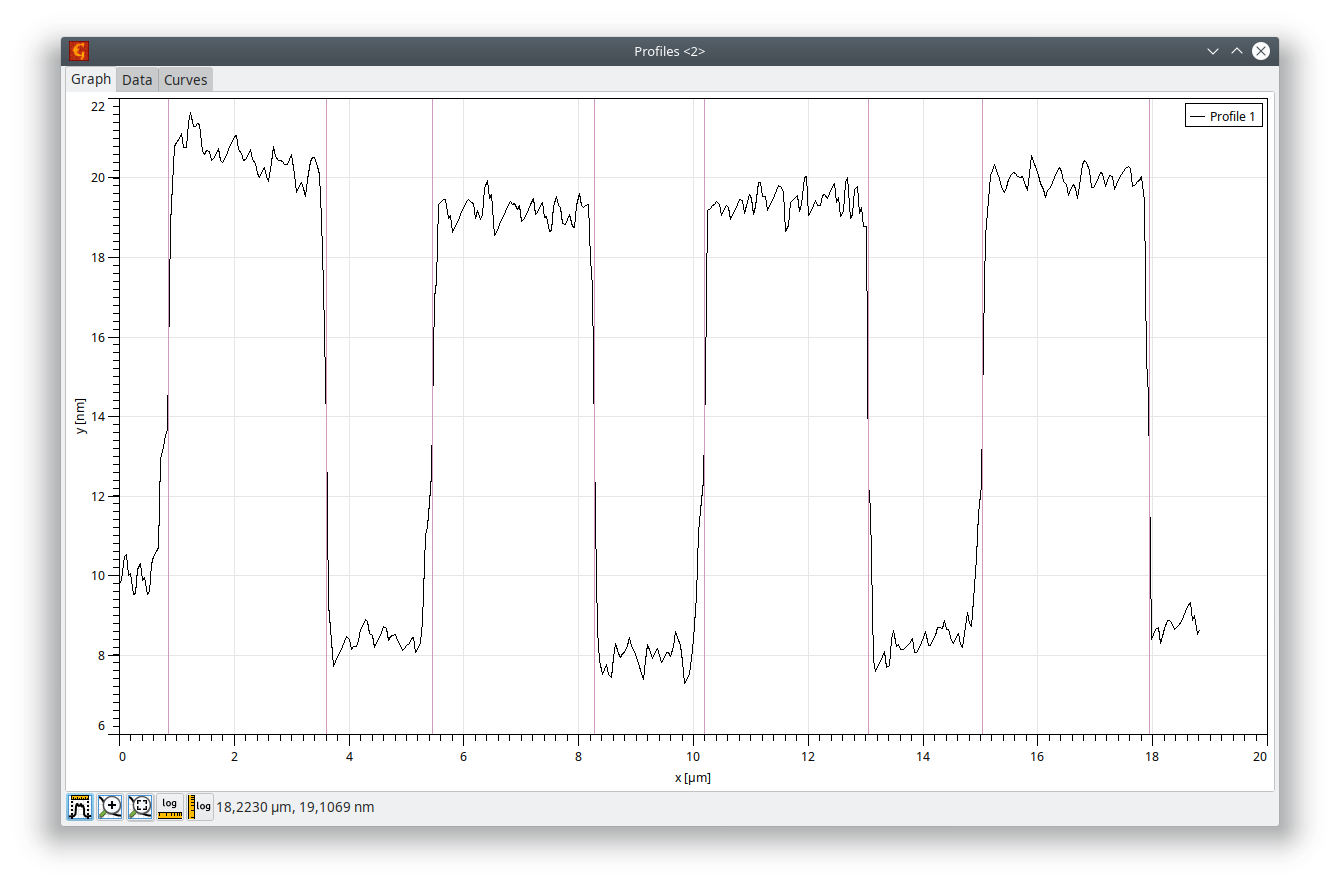
\includegraphics[width=0.6\textwidth]{bilder/Mikrostruktur/LineProfile.png}
    \caption{Linienprofil aufgenommen entlagen der Geometie der Kreisstruktur zur Bestimmung der Abstände in x-Richtung.}
    \label{fig:KREISE3}
\end{figure}

Der Durchmesser der Kreise beträgt im Mittel $(2.82\pm 0.02)\,\si{\micro\meter}$ in x-Richtung und $(3.01\pm 0.03)\,\si{\micro\meter}$ in y-Richtung. Die Periodizizät der gesamtenn Struktur beträgt $(4.87\pm 0.03)\,\si{\micro\meter}$,
dabei wurde sowohl über Vor- wie Rückwärts Scans, alle sichtbaren Kreisstrukturen und x- und y- Richtung gemittelt.

\begin{figure}[H]
    \centering
    \begin{subfigure}{0.49\textwidth}
        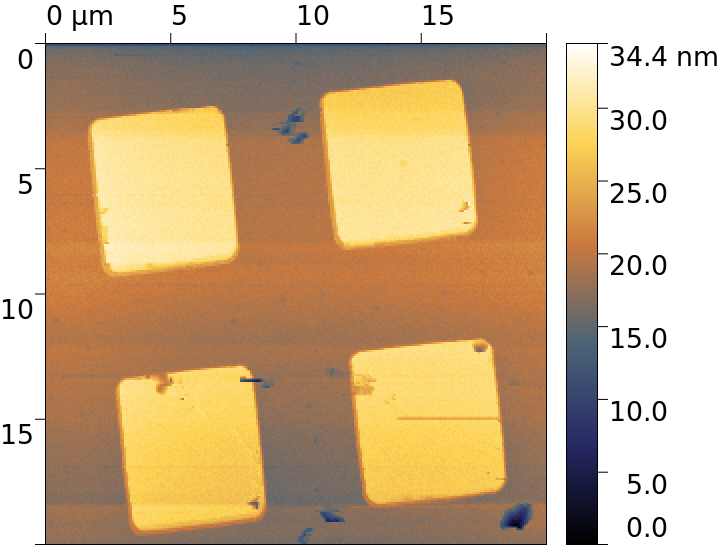
\includegraphics[width=\textwidth]{bilder/Mikrostruktur/Quadrat_Vor_2D.png}
        \caption{}
    \end{subfigure}
    \begin{subfigure}{0.49\textwidth}
        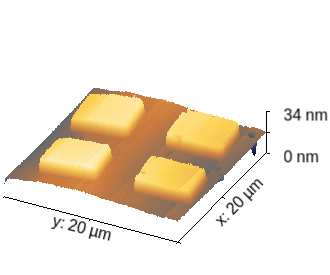
\includegraphics[width=\textwidth]{bilder/Mikrostruktur/Quadrat_Vor_3D.png}
        \caption{}
    \end{subfigure}
    \begin{subfigure}{0.49\textwidth}
        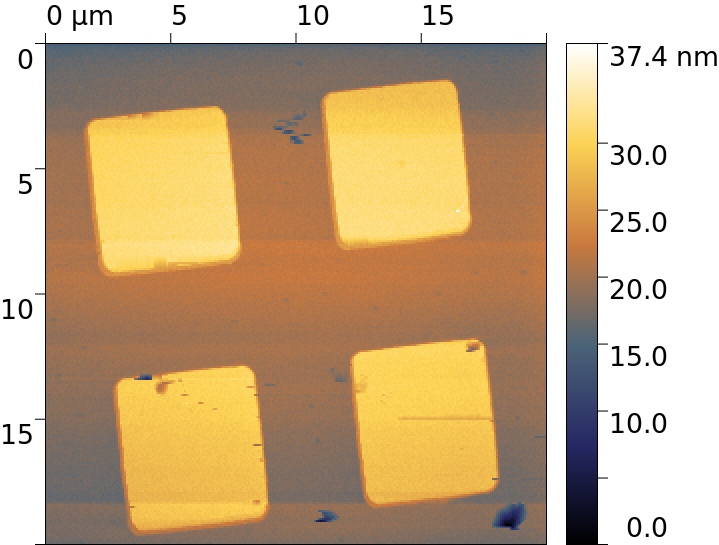
\includegraphics[width=\textwidth]{bilder/Mikrostruktur/Quadrat_Bac_2D.png}
        \caption{}
    \end{subfigure}
    \begin{subfigure}{0.49\textwidth}
        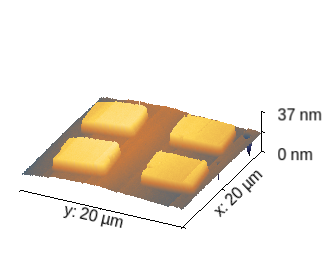
\includegraphics[width=\textwidth]{bilder/Mikrostruktur/Quadrat_Bac_3D.png}
        \caption{}
    \end{subfigure}
    \caption{Mit Gwyddion aufbereitete Daten der Quadratstruktur. \textbf{(a)} Vorwärtsscan in 2D Darstellung, \textbf{(b)} Vorwärtsscan in 3D Darstellung, \textbf{(c)} Rückwärtsscan in 2D Darstellung, \textbf{(d)} Rückwärtsscan in 3D Darstellung.}
    \label{fig:Quadrate}
\end{figure}

In Abbildung \ref{fig:Quadrate} sind die auf die gleiche Weise wie oben aufbereiteten Daten der Quadratstruktur dargestellt.
Auch hier wurden die Strukturabstände mit Linienprofilen vermessen, dabei beträgt die Mittlere Länge eines Quadrats in x-Richtung $(5.79\pm 0.02)\,\si{\micro\meter}$ und in y-Richtung $(6.04\pm 0.03)\,\si{\micro\meter}$.
Die gesamte Struktur ist im Mittel $(9.88\pm 0.04)\,\si{\micro\meter}$ lang. 

\begin{figure}[H]
    \centering
    \begin{subfigure}{0.49\textwidth}
        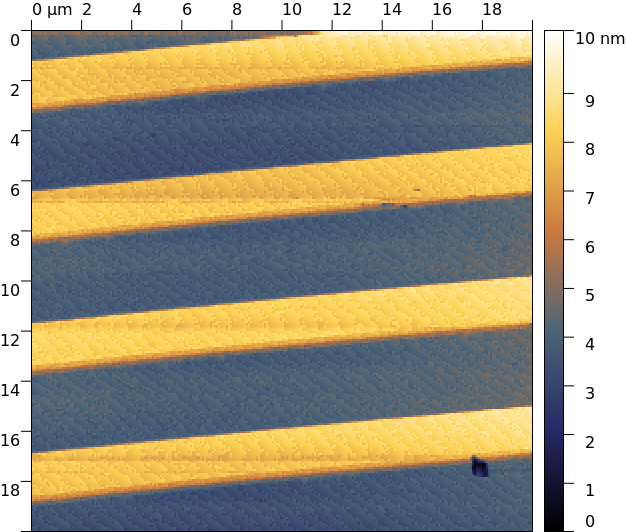
\includegraphics[width=\textwidth]{bilder/Mikrostruktur/Streifen_Vor_2D.png}
        \caption{}
    \end{subfigure}
    \begin{subfigure}{0.49\textwidth}
        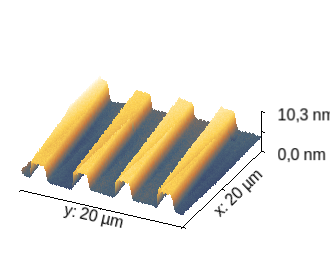
\includegraphics[width=\textwidth]{bilder/Mikrostruktur/Streifen_Vor_3D.png}
        \caption{}
    \end{subfigure}
    \begin{subfigure}{0.49\textwidth}
        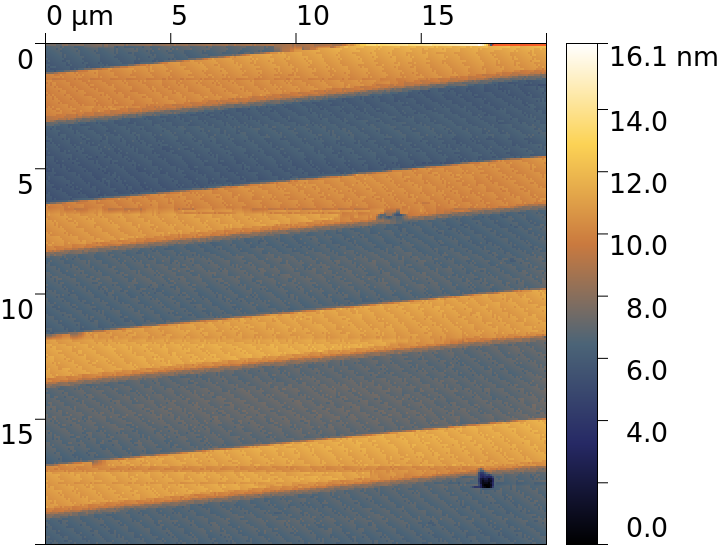
\includegraphics[width=\textwidth]{bilder/Mikrostruktur/Streifen_Bac_2D.png}
        \caption{}
    \end{subfigure}
    \begin{subfigure}{0.49\textwidth}
        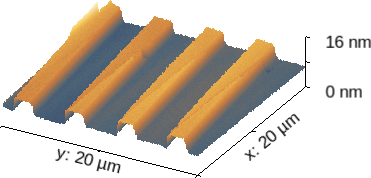
\includegraphics[width=\textwidth]{bilder/Mikrostruktur/Streifen_Bac_3D.png}
        \caption{}
    \end{subfigure}
    \caption{Mit Gwyddion aufbereitete Daten der Streifenstruktur. \textbf{(a)} Vorwärtsscan in 2D Darstellung, \textbf{(b)} Vorwärtsscan in 3D Darstellung, \textbf{(c)} Rückwärtsscan in 2D Darstellung, \textbf{(d)} Rückwärtsscan in 3D Darstellung.}
    \label{fig:Streifen}
\end{figure}

Zuletzt sind in Abbildung \ref{fig:Streifen} die auf die gleiche Weise wie oben aufbereiteten Daten der Streifenstruktur zu sehen.
Auch hier wurden die Strukturabstände mit Linienprofilen vermessen, dabei beträgt die Mittlere Breite eines Streifens $(1.99\pm 0.01)\,\si{\micro\meter}$ und 
die gesamte Struktur ist im Mittel $(5.08\pm 0.02)\,\si{\micro\meter}$ lang. 


%============================================================================================================================

\subsection{CD, DVD und Blu-Ray}

In Abbildung \ref{fig:CD_A} sind die aufgenommenen Daten für eine CD (oben), eine DVD (mitte) und eine Blu-Ray (unten)
als 3D Bild dargestellt. Die Extrahierten Spurbreiten, Spurabstände, minimale und maximale Pitlänge sowie die Pittiefe 
sind in Tabelle \ref{tab:CD1} im Vergleich mit Literaturwerten aufgetragen.

\begin{figure}[H]
    \centering
    \begin{subfigure}{0.49\textwidth}
        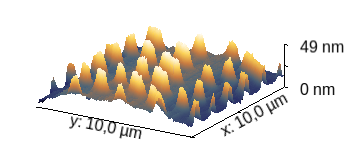
\includegraphics[width=\textwidth]{bilder/CD,DVD,Blu-Ray/CD_s.png}
        \caption{}
    \end{subfigure}
    \begin{subfigure}{0.49\textwidth}
        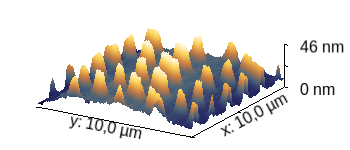
\includegraphics[width=\textwidth]{bilder/CD,DVD,Blu-Ray/CD_Bac_s.png}
        \caption{}
    \end{subfigure}
    \begin{subfigure}{0.49\textwidth}
        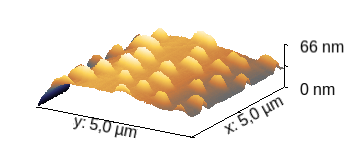
\includegraphics[width=\textwidth]{bilder/CD,DVD,Blu-Ray/DVD_s.png}
        \caption{}
    \end{subfigure}
    \begin{subfigure}{0.49\textwidth}
        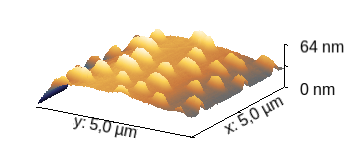
\includegraphics[width=\textwidth]{bilder/CD,DVD,Blu-Ray/DVD_Bac_s.png}
        \caption{}
    \end{subfigure}
    \begin{subfigure}{0.49\textwidth}
        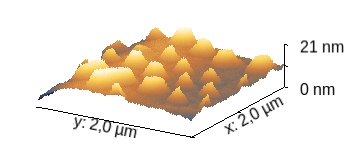
\includegraphics[width=\textwidth]{bilder/CD,DVD,Blu-Ray/Blu-Ray_s.png}
        \caption{}
    \end{subfigure}
    \begin{subfigure}{0.49\textwidth}
        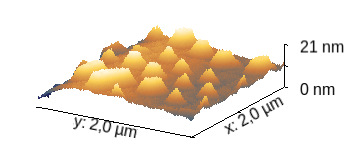
\includegraphics[width=\textwidth]{bilder/CD,DVD,Blu-Ray/Blu-Ray_Bac_s.png}
        \caption{}
    \end{subfigure}
    \caption{Mit Gwyddion aufbereitete Daten verschiedener Datenträger. \textbf{(a)},\textbf{(b)} Bilder der CD, vorwärts und rückwärts. \textbf{(c)},\textbf{(d)} Bilder der DVD, vorwärts und rückwärts. \textbf{(e)},\textbf{(f)} Bilder der Blu-Ray, vorwärts und rückwärts.}
    \label{fig:CD_A}
\end{figure}

\begin{table}
    \centering
    \makebox[\textwidth][c]{
    \begin{tabular}{c| c c c c c}
    \toprule
    \textbf{CD} &Spurbreite [$\si{\micro\meter}$]&Spurabstand [$\si{\micro\meter}$]&min Pitlänge [$\si{\micro\meter}$]&max Pitlänge [$\si{\micro\meter}$]&Pittiefe [$\si{\nano\meter}$]\\
    \midrule
    Messwert &$0.46\pm0.01$&$1.52\pm0.02$&$0.78\pm0.02$&$2.22\pm0.06$&$24.8\pm0.3$\\
    Literaturwert & $0.5$ & $1.6$ & $0.833$ & $3.054$ & $100$ \\
    Abweichung & $6.0\,\si{\percent}$ & $3.8\,\si{\percent}$ & $4.0\,\si{\percent}$ & $25.3\,\si{\percent}$ & $74.9\,\si{\percent}$ \\
    \midrule
    \midrule
    \textbf{DVD} &Spurbreite [$\si{\micro\meter}$]&Spurabstand [$\si{\micro\meter}$]&min Pitlänge [$\si{\micro\meter}$]&max Pitlänge [$\si{\micro\meter}$]&Pittiefe [$\si{\nano\meter}$]\\
    \midrule
    Messwert &$0.24\pm0.04$&$0.73\pm0.02$&$0.42\pm0.02$&$1.105\pm0.003$&$13.5\pm0.2$\\
    Literaturwert & $0.2$ & $0.74$ & $0.4$ & $1.87$ & $102.8$ \\
    Abweichung & $-$ & $-$ & $-$ & $40.7\,\si{\percent}$ & $86.7\,\si{\percent}$ \\
    \midrule
    \midrule
    \textbf{Blu-Ray} &Spurbreite [$\si{\micro\meter}$]&Spurabstand [$\si{\micro\meter}$]&min Pitlänge [$\si{\micro\meter}$]&max Pitlänge [$\si{\micro\meter}$]&Pittiefe [$\si{\nano\meter}$]\\
    \midrule
    Messwert&$0.129\pm0.009$&$0.371\pm0.004$&$0.117\pm0.009$&$0.494\pm0.002$&$6.50\pm0.08$\\
    Literaturwert & $0.13$ & $0.32$ & $0.149$ & $0.695$ & $64.1$ \\
    Abweichung & $-$ & $14.7\,\si{\percent}$ & $15.4\,\si{\percent}$ & $28.6\,\si{\percent}$ & $89.7\,\si{\percent}$ \\
    \bottomrule
    \end{tabular}
    }
    \caption{Extrahierte Daten über Spurbreite, Spurabstand, minimale, sowieso maximale Pitlänge und Pittiefe für die CD, DVD und Blu-Ray. Außerdem sind Literaturwerte \cite{CD}\cite{DVD}\cite{DVD2}\cite{Blu-Ray} aufgetragen und die Abweichungen der gemessenen Werte von den Literaturwerten. Bei fehlendem Eintrag ('-') liegt der Literaturwert im Unsicherheitsintervall des Messwerts.}
    \label{tab:CD1}
\end{table}

Erwartet wird eine Pittiefe von einem viertel der Wellenlänge des auslesenden Lasers im Medium (Brechungsindex beachten).
Beim zweimaligen Durchlaufen des Materials ergibt sich so genau ein Gangunterschied von einer halben Wellenlänge des Lasers.
Zuletzt wird noch die Speicherkapazität der CD bestimmt. Dabei entspricht der kürzeste Pit 4 Bit \cite{anleitung}. Mit Hilfe des Spurabstandes 
$(1.52\pm0.02)\,\si{\micro\meter}$ lässt sich so eine Bitdichte von $(3.37\pm0.09)*10^{12}\,\text{Bit}/\si{\meter\squared}$ errechnen. Der beschreibbare Teil einer CD ist $0.0089\,\si{\meter\squared}$ groß \cite{CD_Größe}, somit können auf einer CD
insgesammt $(3.00\pm0.08)*10^{10}$ Bits gespeichert werden. Ein Byte setzt sich aus 
14 Bit + 3 Trennbit zusammen \cite{anleitung}, somit ergeben sich $(1.77\pm0.05\,)$GB.

%============================================================================================================================

\subsection{Kraft-Abstandskurven}

Da die Berechnungen primär die auftretenden Größenordnungen aufzeigen sollen \cite{anleitung},
werden in diesem Abschnitt keine Fehlerrechnungen durchgeführt.
Die aufgenommenen Kraft-Abstandskurven sind in den Abbildungen \ref{fig:Edel} \ref{fig:Kraft} zu sehen.
Beispielhaft ist die Kurve für Edelstahl beschriftet. Zunächst wird die Probe der Spitze angenähert (Blau), wobei 
Probe und Spitze nicht in Kontakt stehen. Beim "Snap-in" ist der Kontakt hergestellt.
Bei weiterer Annäherung steigt die Ablenkungsspannung linear zur z piezo Spannung.
Beim zurückfahren der Probe (rot) kommt es beim Ende des Kontakts zum "Pull-off", bei dem 
die Spitze sich von der Probe löst. Danach entfernt die Probe sich ohne Kontakt weiter von der Spitze.
\begin{figure}[H]
    \centering
    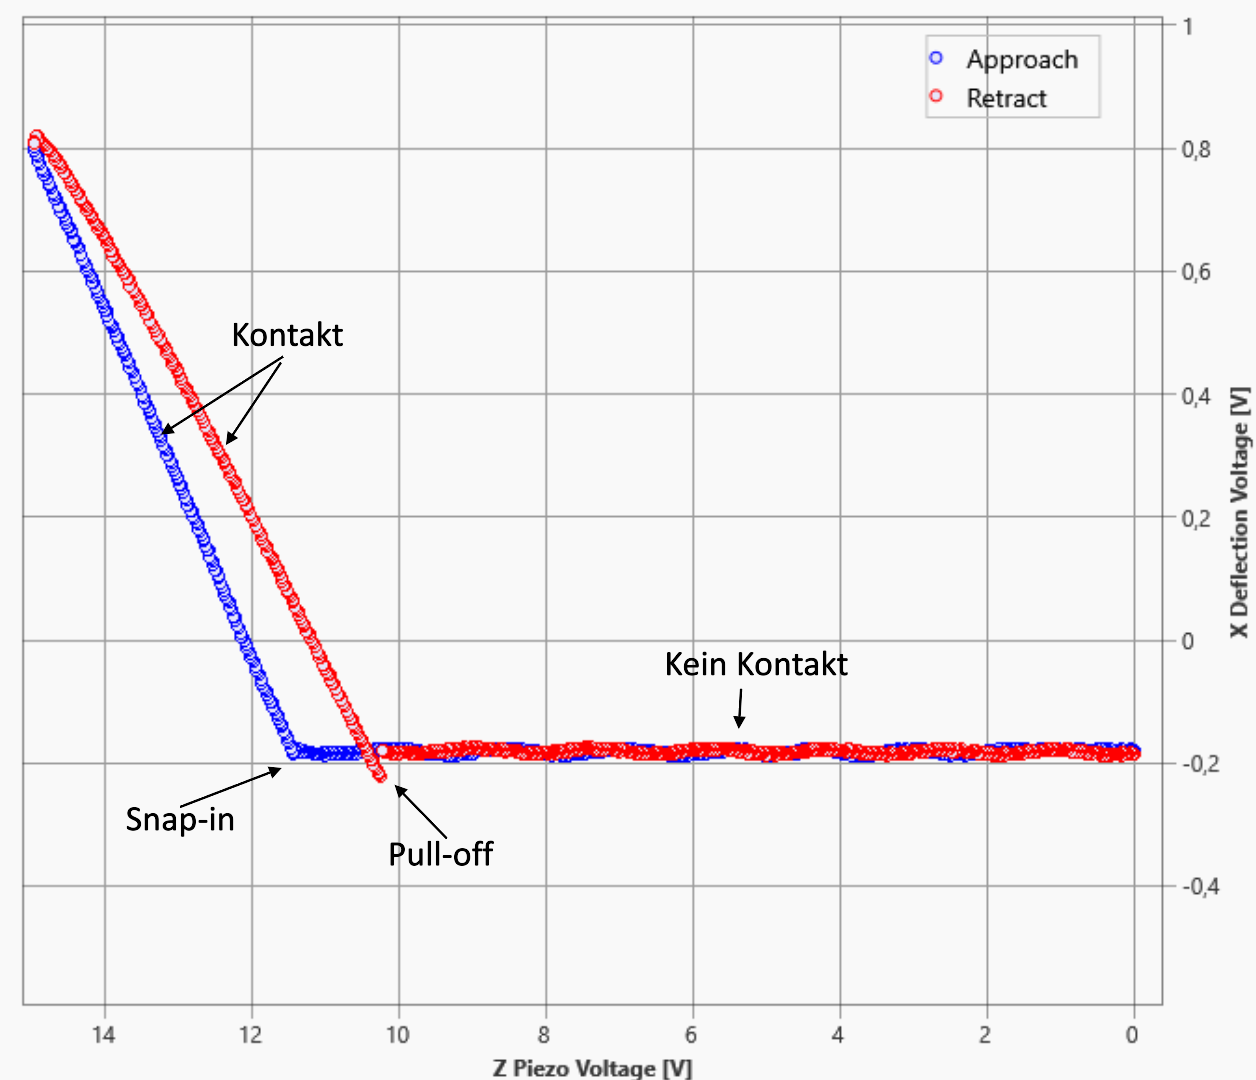
\includegraphics[width=0.7\textwidth]{bilder/Kraft_Abstand/Beschriftet_Edelstahl.png}
    \caption{Gemessene und beschriftete Kraft-Abstandskurve von Edelstahl.}
    \label{fig:Edel}
\end{figure}

\begin{figure}[H]
    \centering
    \begin{subfigure}{0.49\textwidth}
        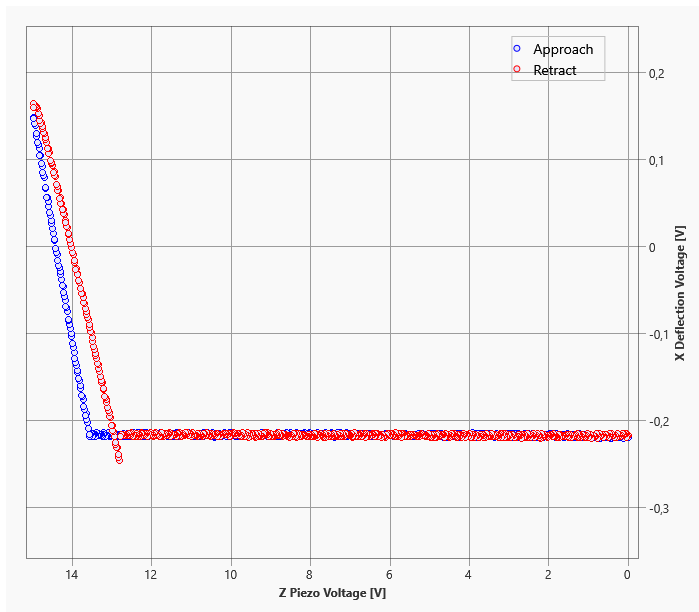
\includegraphics[width=\textwidth]{bilder/Kraft_Abstand/FDC_Si.png}
        \caption{}
    \end{subfigure}
    \begin{subfigure}{0.49\textwidth}
        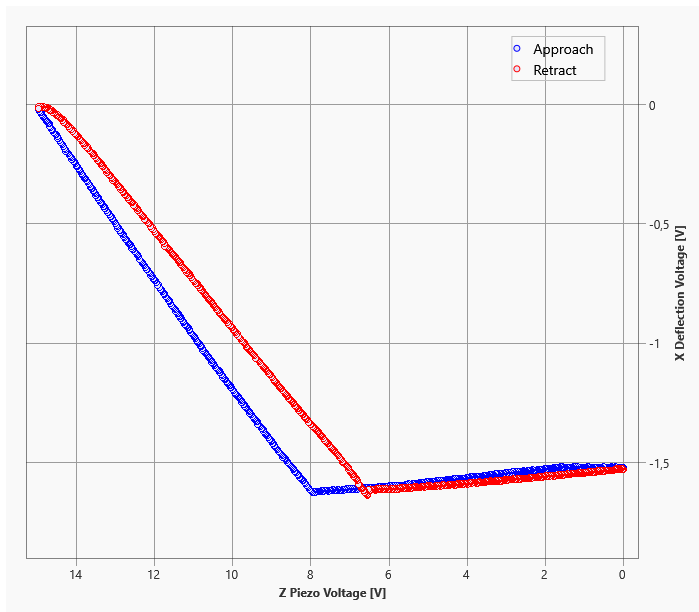
\includegraphics[width=\textwidth]{bilder/Kraft_Abstand/FDC_Teflon.png}
        \caption{}
    \end{subfigure}
    \caption{Gemessene Kraft-Abstandskurven für \textbf{(a)} Silizium und \textbf{(b)} Teflon.}
    \label{fig:Kraft}
\end{figure}

Aus den Z Piezo Spannungen des Snap-in und Pull-off lassen sich mit dem Umrechnungsfaktor $\frac{20\,\si{\micro\meter}}{75\,\si{\volt}}=0.267\,\si{\micro\meter\per\volt}$ \cite{anleitung}
eine Höhendifferenz zwischen Snap-in und Pull-off berechnen. Für die Berechnung der Adhäsionskraft wurde die Federkonstante $k=0.2\,\si{\newton\per\meter}$ \cite{anleitung} verwendet.
Die Ergebnisse dieser Rechnungen sind in Tabelle \ref{tab:KraftAbstand} eingetragen.

\begin{table}
    \centering
    \makebox[\textwidth][c]{
        \begin{tabular}{c| c c c c}
        \toprule
        \textbf{Material} &Snap-in [$\si{\volt}$]&Pull-off [$\si{\volt}$]&Höhendifferenz [$\si{\micro\meter}$]&Adhäsionskraft [$\si{\nano\newton}$]\\
        \midrule
        Edelstahl & $11.475$ & $10.256$ & $0.325$ & $65$\\
        Silizium & $13.594$ & $12.806$ & $0.210$ & $42$\\
        Teflon & $7.988$ & $6.544$ & $0.386$ & $77$\\
        \bottomrule
        \end{tabular}
    }
    \caption{Ermittelte Werte für Snap-in und Pull-off für Edelstahl, Silizium und Teflon. Außerdem sind die errechneten Werte für die Höhendifferenz und die Adhäsionskraft eingetragen.}
    \label{tab:KraftAbstand}
\end{table}

Für die Berechnung des Elastizitätsmoduls von Teflon wird zunächst die Kraft

\begin{equation}
    F=\frac{2}{\pi}\tan(\alpha)E^*\rho^2
\end{equation}

betrachtet, mit der die Spitze auf die Probe drückt. Dabei wird angenommen, dass die Spitze eine Kegelform hat.
$\alpha$ bezeichnet hierbei den halben Öffnungswinkel der Cantileverspitze, der laut Quelle \cite{anleitung} $\alpha=10\,\si{\degree}$ beträgt.
$\rho$ bezeichnet die Eindringtiefe der Spitze in die Oberfläche und $E^*$ die oberflächenelastische Konstante

\begin{equation}
    E^*=\frac{E}{1-\nu^2},
\end{equation}

mit der Poissonzahl $\nu$ und dem Elastizitätsmodul $E$ \cite{Elasti}. Die Poissonzahl wird für Teflon als $\nu=0.46$ bei $23\,\si{\celsius}$ in der Literatur angegeben \cite{P}.
Somit lassen sich diese Gleichungen umformen zu

\begin{equation}
    E=\frac{F\pi(1-\nu^2)}{2\tan(\alpha)\rho^2},
\end{equation}

wobei die Eindringtiefe der Spitze in die Teflon-Oberfläche $\rho$ und die Kraft $F$, mit der die Spitze auf die Probe drückt, aus den Messdaten bestimmt werden muss.
Letzteres kann wie bei der Adhäsionskraft mittels der Federkonstanten und der Auslenkung des Cantilevers bestimmt werden.
Für die Eindringtiefe wird die Auslenkung des Cantilevers bei dieser Spannung mit der Auslenkung des Cantilevers bei einer undeformierbaren Probe, hier Edelstahl, verglichen.
Die Differenz der Auslenkungen entspricht dann der Eindringtiefe des Cantilevers in die Teflon-Oberfläche.

Bei einer Z Piezo Spannung von $3.506\,\si{\volt}$ über dem Snap-in,
beträgt die X-Ablenkung Spannung $0.765\,\si{\volt}$ über dem Snap-in bei der Teflon Probe.
Den gleichen X-Ablenkung Spannungs Wert über dem Snap-in hat die Edelstahlprobe bei einem z Piezo Spannungswert von $2.719\,\si{\volt}$ über dem Snap-in.
Aus der Differenz lässt sich so eine Eindringtiefe von $\rho=0.210\,\si{\micro\meter}$ berechnen.
Die Kraft $F$ lässt sich wie oben mit der Federkonstanten von $k=0.2\,\si{\newton\per\meter}$ zu $F=145\,\si{\nano\newton}$ berechnen.
Insgesammt ergibt sich so ein Elastizitätsmodul von $23.12\,\si{\mega\pascal}$.